\documentclass[conference]{IEEEtran}
\IEEEoverridecommandlockouts
% The preceding line is only needed to identify funding in the first footnote. If that is unneeded, please comment it out.
\usepackage{cite}
\usepackage{amsmath,amssymb,amsfonts}
\usepackage{tikz}
\usetikzlibrary{arrows.meta, positioning}
\usepackage{hyperref}
\usepackage{algorithmic}
\usepackage{graphicx}
\usepackage{textcomp}
\usepackage{xcolor}
\usepackage{xurl}
\def\BibTeX{{\rm B\kern-.05em{\sc i\kern-.025em b}\kern-.08em
    T\kern-.1667em\lower.7ex\hbox{E}\kern-.125emX}}
\begin{document}

\title{ Kernel - Level Semantic Search with Knowledge Graphs
}

% \author{\IEEEauthorblockN{\textsuperscript}
% \and
% \IEEEauthorblockN{Arjun Deodhar}

% \IEEEauthorblockA{\textit{COEP Technological University} \\
% Dept. of Computer Science\\
% % \textit{COEP}\\
% Pune, Maharashtra\\
% deodhark22.comp@coeptech.ac.in}
% \and
% \IEEEauthorblockN{Arnav Prasad}
% \IEEEauthorblockA{\textit{COEP Technological University} \\
% Dept. of Computer Science\\
% % \textit{COEP}\\
% Pune, Maharashtra \\
% arnavp22.comp@coeptech.ac.in}
% \and
% \IEEEauthorblockN{Prajwal Bhosale}
% \IEEEauthorblockA{\textit{COEP Technological University} \\
% % \textit{COEP}\\
% Dept. of Computer Science\\
% Pune, Maharashtra\\
% bhosalepp22.comp@coeptech.ac.in}
% }

\author{\IEEEauthorblockN{}
\and
\IEEEauthorblockN{Arjun Deodhar}
\IEEEauthorblockA{\textit{Department of Computer Science} \\
\textit{COEP Technological University} \\
Pune, Maharashtra, India \\
deodhark22.comp@coeptech.ac.in} 
\and
\IEEEauthorblockN{Arnav Prasad}
\IEEEauthorblockA{\textit{Department of Computer Science} \\
\textit{COEP Technological University} \\
Pune, Maharashtra, India \\
arnavp22.comp@coeptech.ac.in}
\and
\IEEEauthorblockN{Prajwal Bhosale}
\IEEEauthorblockA{\textit{Department of Computer Science} \\
\textit{COEP Technological University} \\
Pune, Maharashtra, India \\
bhosalepp22.comp@coeptech.ac.in}
}


\maketitle

\begin{abstract}
Various types of knowledge exists across individuals, processes and tools.
The chief objective of Knowledge Graph (KG) is to aggregate the data into graph format, ensuring that it remains manageable, non-corrupted, scalable and easily discoverable.

At its core, a KG is a structure were each node represents real-world entities and edges logically depict the relationships between the nodes. The graph can either be directed or un-directed, depending on the organization's need. Our approach involves a directed graph that also includes backward edges!

The end objective of KG is to operationalize Knowledge (a piece of information) at the kernel level and make it available to users when they feed specific queries to the graph. The output should be the most relevant and concise response available, neither too lengthy nor too brief.
\end{abstract}

% \begin{IEEEkeywords}
% Knowledge Graphs, AVL, heap
% \end{IEEEkeywords}

\subsection{Abbreviations and Acronyms}\label{AA}

\begin{itemize}
    \item \textbf{KGs}: Knowledge Graphs
    \item \textbf{AVL}: Adelson-Velsky and Landis
    \item \textbf{max\_heap}: maximum heap
    \item \textbf{NLP}: Natural Language Processing
    \item \textbf{LLM}: Large Language Model
\end{itemize}




\section{Introduction}
KGs are advanced data structures that represent information in a network of interconnected entities and their relationships. They consist of nodes, representing entities (such as people, places, or concepts) and edges, representing the relationships between these entities. They are designed to enable machines to understand and process complex data, facilitating improved information retrieval, question answering, and semantic search capabilities.
The concept of the KG gained significant recognition in 2012 when Google \cite{b7} publicly credited their search solution to the use of KG.
The relationships in KG are often labeled to provide context and meaning, forming a rich, structured representation of knowledge.
One of the key advantages of KGs is their ability to integrate and organize data from various sources, providing a unified view that can be easily queried and analyzed. They support both direct and inferred relationships, enabling more sophisticated reasoning and inference.
\\KGs have various applications : 
\begin{itemize}
    \item \textbf{E-Commerce}: Widely used by platforms like Amazon\cite{b2, b3} and eBay\cite{b4} to describe and categorize products for sale.
    \item \textbf{Social Networking}: Utilized by platforms such as LinkedIn\cite{b5} to manage and connect users, jobs, skills, and more.
    \item \textbf{Finance}: Bloomberg\cite{b6} has developed a KG that powers financial data analytics, including sentiment analysis for companies based on current news reports and tweets.
\end{itemize}

This paper focuses on the structural implementation of a KG. It takes input from users and serves as a critical source of knowledge across various domains. 
\\
The primary contributions of this study are summarized as follows:

\begin{itemize}
    \item It introduces a structural framework for constructing a KG at the kernel level without relying on external libraries.
    \item The developed KG can manage diverse types of queries, providing precise and relevant responses.
\end{itemize}
% The goal of this tutorial paper is to motivate and guide a comprehensive introduction to core implementation of KG.
The aim of this paper is to provide a road-map for a thorough exploration of the fundamental implementation aspects of KGs.


\section{Literature Survey}

A primary reference for our study was the paper "Knowledge Graphs"\cite{b8} by Aidan Hogan et al. The paper features a rich bibliography with over 400 references, providing detailed explanations on KG concepts such as graph modeling, ontologies, deductive knowledge, graph embeddings and more. 

The paper "The Potential of the PID Graph" \cite{b16} presented and highlighted the concept and importance of "identity" in the context of data parsing and extraction(as discussed in section..).

The paper "Context-Aware Temporal Knowledge Graph Embedding" \cite{b17} examined the concept of temporal context (as discussed in section ..).


% Our exploration identified RDF (Resource Description Framework) [1] as a prominent data-modeling language used in KG design. Other notable languages encountered include SPARQL [10] and Neo4j [11]. Additionally, we reviewed a comprehensive paper on the foundations of modern query languages for graph databases [12].

With reference to \cite{b8}, we studied various graph models, including heterogeneous graphs\cite{b18}, property graphs\cite{b12}, and directed-edge labelled graphs\cite{b8}. This paper delves into the implementation of directed-edge labelled weighted graphs with further additions and improvements.

"Introduction to Algorithms" \cite{b14} provided the knowledge needed to select the appropriate data structures and efficient algorithms. "The C Programming Language" \cite{b9} was used to implement these algorithms in C.

These insights from the literature review, inspired the authors to present the structural implementation and significance of KGs

\section{Methodology}
Data includes a wide range of scope and context. It can be of variable length, contexts, grammars, etc.
A KG is not just a collection of data, but also contains hierarchical structures, contexts for data, as well as unique identifiers for real word \cite{b8}
\\
The constructed KG should be able to handle and recognize the following characteristics of data:
\begin{itemize}
    \item\textbf{Context of entities.}\cite{b8}\\ 
    For example, if the word "bank" is considered, the context can be river-side bank or the bank which involves financial transactions or specifically Bank of Maharashtra or may have some other context.
    

    
	\item\textbf{Weight of the connection}
 \\
 The connection with highest weight should be displayed first.
 \\
 This includes recognition of "front-weight" and "back-weight" of data. For example, consider the sentence : "Arjun plays piano". This may be an important attribute for "Arjun" but not that relevant for "piano"(i.e. piano is being played by "Arjun" and piano will have more important(weighted) characteristics). The text analyzer should be able to assign front and back weights accordingly.

 
	\item\textbf{Temporal constraints} \cite{b8, b17}
 \\
 For example, the statement "XYZ is the Prime Minister of India" will be valid only for a certain period of time(say five years) and then it may change. After expiration, the relation should be redundant.

 
	\item\textbf{Identity} \cite{b8,b16}
 \\
 For example, "Arjun plays piano" and "Arjun plays guitar", although the name "Arjun" has been repeated, but in the real world it may refer to different entities. 
 The analyzer should assign unique identifiers to different entities.
	
 \item\textbf{Misspelled Words Queries} 
 \\
 The query analyzer should be able to detect spelling errors in input queries and deliver the correct output by prompting the matching entities.
 
\end{itemize}

To accomplish all these features, the designed input data set contains the following fields: front-weight, inference, truth-bit, noun1, noun1\_id , verb , verb descriptor, noun2, noun2\_id, back-weight, definition, end-time.




\section*{IV. ARCHITECTURE}

\subsection{Data Structures Used}
The implementation in C programming language\cite{b9}, employs structures and pointers for AVL trees and arrays for heaps, providing a robust framework for managing noun-centric knowledge representations and their interconnections via verbs.

\subsubsection{AVL Tree}

AVL trees\cite{b14} are among the most efficient data structures for searching and inserting nodes(data) due to their 
self-balancing nature. The predictable performance of AVL trees makes 
them a powerful and widely used choice in computer 
science.
They are particularly used in scenarios requiring fast and reliable search operations such as database indexing.

The insertion and search operations in an AVL tree have a time complexity of $O(\lg n)$, 
where "n" represents the number of nodes already present in the AVL tree.


\subsubsection{Maximum Heap}

Max\_heaps\cite{b14} are highly efficient data structures for managing and retrieving the maximum weighted element . 
They maintain a structure similar to the complete binary tree structure, ensuring that the most weighted 
element is always at the root, which allows for constant time retrieval of the maximum value.
It enables $O(1)$ time complexity for retrieval.

Inserting and deleting elements in a max heap is efficient, with both operations having $O(\lg n)$ 
   time complexity.

All these make Max\_Heap quite useful in applications like scheduling algorithms,resource management 
and real-time simulations.


\subsection{Structural Implementation}

\subsubsection{\textbf{Central Noun Tree}}
The core of our KG is an AVL tree where each node represents a noun. Each noun node comprises the following elements:
\begin{itemize}

    \item \textit{noun\_name}: Pointer to a string representing the noun.
    \item \textit{noun\_id}: A unique identifier for the noun.
    \item \textit{noun\_definition}: Pointer to a string containing the definition of the noun.
    \item \textit{next\_verb\_tree}: An AVL tree containing verbs that form front links to other nouns.
    \item \textit{prev\_verb\_tree}: Pointer to an AVL tree containing verbs that form back-links to other nouns.
    \item \textit{search\_max\_heap}: A max\_heap for extracting the highest priority connections.
    \item \textit{subclass\_max\_heap}: A max\_heap for accessing the highest priority sub-classes of the noun.
    \item \textit{left, right, balance\_factor} : for maintaining AVL tree. 
    
\end{itemize}

\begin{figure}[htbp]
\centering
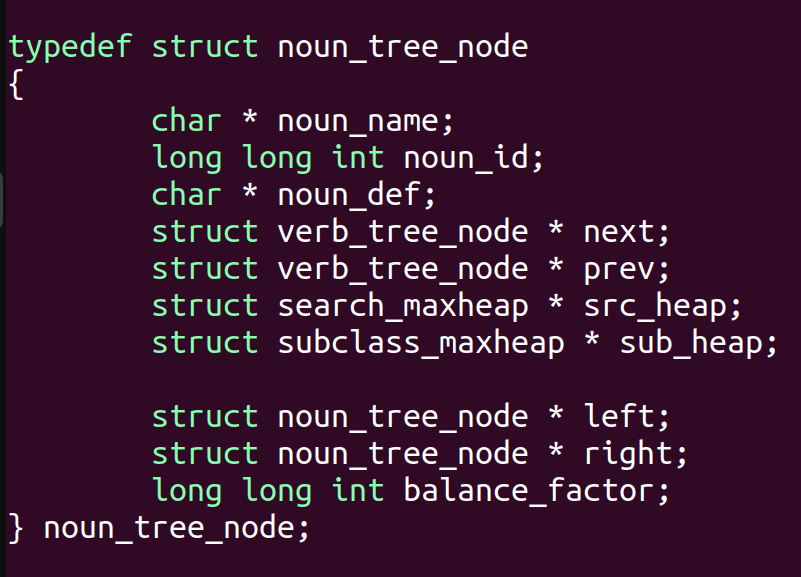
\includegraphics[width=0.8\linewidth]{c1.png} % Adjust the width as needed
\caption{Structural implementation in C}
\label{fig}
\end{figure}


\begin{figure}[htbp]
\centering
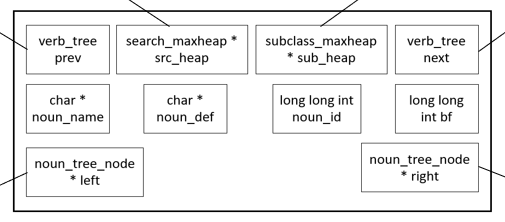
\includegraphics[width=0.8\linewidth]{fig_2_2.png} % Adjust the width as needed
\caption{Figure shows Structure diagram for Central Noun Tree node.}
\label{fig}
\end{figure}

\subsubsection{\textbf{Prev and Next Verb Trees}}
As explained previously, each noun\_tree node has its own next and previous verb\_trees. These contain connections to edges as well as some information about the verb being stored
Each verb\_tree node comprises of:
% char * verb_name;
%         struct query_maxheap* qheap;
%         struct verb_tree_node * left;
%         struct verb_tree_node * right;
%         long long int bf;

\begin{itemize}

    \item \textit{verb\_name}: Pointer to a string in the database tree of verbs
    \item \textit{qheap}: A max\_heap that contains essential edge information
    \item \textit{left, right, balance\_factor}:for maintaining AVL tree. 
    \item \textit{next\_verb\_tree}: An AVL tree containing verbs that form front links to other nouns.
    
\end{itemize}

\subsubsection{\textbf{Verb Database Trees}}
Two additional AVL trees are maintained to store:
\begin{itemize}
    \item verbs.
    \item verb descriptors.
\end{itemize}
These database trees serve as storage repositories to efficiently reuse allocated string memory. 
For example, if the verb "plays" occurs in multiple input lines, then memory for the string "plays" will be allocated only once and all references to "plays" will eventually point to the same memory location. 
Nodes in these trees are not interconnected, focusing solely on memory optimization.

\subsubsection{\textbf{Sub-class Max\_heap}}
This includes the sub-classes of the noun. For example, animal\_python,animal\_human and animal\_lion will be sub-classes of animal  
\begin{itemize}
    \item A pointer to the target noun node.
    \item \textit{weight}: The importance of the subclass.
\end{itemize}

\begin{figure}[htbp]
\centering
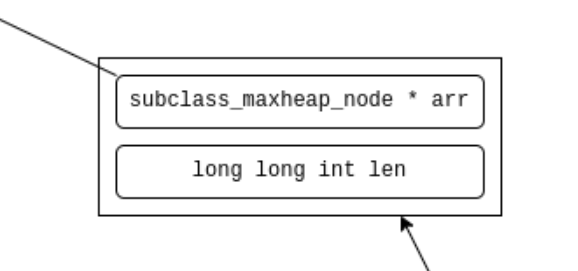
\includegraphics[width=0.8\linewidth]{subclass_maxheap.png} % Adjust the width as needed
\caption{Figure illustrates the Structure of Sub-class Max\_heap.}
\label{fig}
\end{figure}

\\

\subsubsection{\textbf{Edge Representation, search max\_heaps}}
Edges encapsulate the relationships between noun nodes. They are stored in the \textit{query\_max\_heap} of the verb nodes. Each edge contains:
\begin{itemize}

    \item \textit{noun\_ptr} : A pointer to the target noun node.
    \item \textit{truth\_bit}: A boolean indicating the truthfulness of the connection.
    \item \textit{end\_time}: The validity period of the connection.
    \item \textit{weight}: The significance of the connection.
\end{itemize}

\textit{Search\_max\_heap} nodes point to these edges.
//
\begin{figure}[htbp]
\centerline{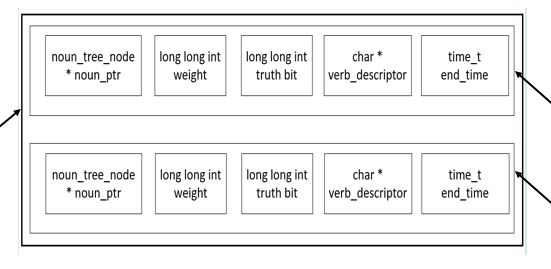
\includegraphics[width=0.5\textwidth]{fig_4_2.png}}
\caption{Figure illustrates the Structure of Edge.}
\label{fig}
\end{figure}



\section{WorkFlow}
\subsection{Example of Entry Creation in the KG}

This section will illustrate how an entry is made in the KG.
For the input line : "Computer Science includes wide range of
Data Structures."

Here, the parser will identify "Computer Science" as "noun1" (first noun of the sentence)
and "Data Structures" as "noun2" (second noun of the given input sentence).
Phrases like "includes" will be classified as "verb" and "wide range of" will be classified as "verb-descriptors".

Now there comes a need to store this sentence into the memory where our structural concept
of KG comes into use.
noun1 and noun2 (i.e., "Computer Science" and "Data Structures") will be inserted into the central AVL noun
tree (explained in section ....).

A new noun i.e., noun3 also gets formed: i.e., noun1 + "\_" + noun2 i.e., "Computer Science\_Data Structures"
and will be inserted in the central AVL tree (reason prescribed in section ...).

Each noun should only be inserted if it does not already exist in the central AVL tree. 
This prevents duplicates, ensuring no redundant nouns are stored, thus optimizing memory usage.

If the noun already exists, connections will be made through the existing noun itself.

The verb "includes" and verb descriptor "wide range of" are also stored in a similar manner
in the Verb Tree and Verb descriptor Tree (explained in section ....).

Further, irrespective of which branch of the central AVL tree the noun gets inserted, 
the connections among them are made, i.e.:

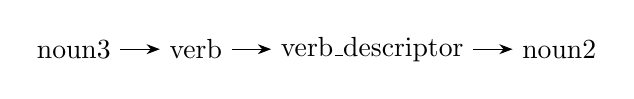
\begin{tikzpicture}[node distance=1.5cm, >=Stealth]
    \node (noun3) {noun3};
    \node (verb) [right=0.5cm of noun3] {verb};
    \node (verb_descriptor) [right=0.5cm of verb] {verb\_descriptor};
    \node (noun2) [right=0.5cm of verb_descriptor] {noun2};

    \draw[->] (noun3) -- (verb);
    \draw[->] (verb) -- (verb_descriptor);
    \draw[->] (verb_descriptor) -- (noun2);
\end{tikzpicture}

(explained in section ....)

In instances where the input line "Computer Science includes a wide range of Data Structures." is 
repeated, instead of creating new connections, the weights associated with the existing connections 
are incremented. This ensures that no redundant data and connections are stored.

This structure helps maintain the relationships within the KG, 
ensuring that each entry is efficiently organized and connected.


\subsection{Output Extraction and Querying the KG}

As an end-user, one may seek the most relevant response to their query. Users might ask questions such as:
\begin{itemize}
    \item "Computer Science includes?"
    \item "? includes Data Structures"
    \item "Computer Science includes Data Structures: True or False?"
    \item Or broader queries like: "Describe Computer Science" or "Computer Science?"
\end{itemize}

Queries may also contain spelling errors, requiring the system to provide the most relevant output and potentially prompt the user with a "Did you mean?" suggestion.
\\
For example, if a user inputs: "Comptr Science includes?" 
\\the system should prompt:
\\
"Did you mean: Computer Science includes?" 
\\
and proceed based on the user's response.
\\

As developers, it is crucial to handle all these types of queries efficiently. Therefore, functions like \texttt{display\_info\_lines} and \texttt{print\_info\_lines} are used, which are detailed in subsequent sections.
\\

Responding to questions like "Describe Computer Science" could overwhelm the user with an extensive amount of data, as the KG may contain thousands of entries related to Computer Science. \\
To manage this, the algorithm prompts the user with a follow-up question: "How many lines of information do you need?" If the user specifies 10 lines, the system will display the 10 most important and weighted connections. 
\\
There is also an option for the system to display all connections in decreasing order of their weights.


\section{Querying and Traversal}


The approach for traversing the KG is "Weight Proportional Breadth-First 
Traversal."

User can shoot their desired queries in an interactive manner. 

Suppose the KG receives the input "Computer Science includes ?" and the user requests: "I want 10 lines of data."
In the KG, data is stored (only necessary details shown, to give an overview) as depicted in the figure:

\begin{figure}[htbp]
\centering
\includegraphics[width=0.8\linewidth]{kg_lines_explained.png} % Adjust the width as needed
\caption{Figure illustrates an example for graph traversal}
\label{fig}
\end{figure}

The dotted line "returns 0" is not a connection, and is rather a function call's return value

Although the KG may contain thousands of connections, for simplicity, let's assume it has three direct connections.

Given the limited number of lines to be displayed, the KG will prioritize the connections based on their weights using a max heap structure and will allocate ratios to the nouns of the next connections. In this case, the proportion is 3 : 2 : 1 
because the weights of the connections are in the ratio 3 : 2 : 1 (i.e., Data Structures, Programming Language, Interesting). The allowed lines will be distributed to the next nodes in these proportions, and this process will continue recursively until all the requested lines have been displayed.\\

\texttt{display\_info\_lines} is the recursive function that is used for this purpose



\subsection{\textbf{\texttt{display\_info\_lines}}}

This function takes
\begin{itemize}
\item \textit{input\_noun} : A string whose connections are to be displayed
\item \textit{total\_lines} : The maximum number of lines to be printed. 
\end{itemize}


\texttt{display\_info\_lines} does:

1) Search for \textit{input\_noun} : Search for the noun in the noun tree of the KG. This search is done to find a 100\% matching string.

If a perfect match isn't found, then another search is done, which gathers all nouns that are matching more than a certain threshold, and an array of choices is generated from this traversal

2) \textit{Display array of choices}: This is displayed as a "did you mean : " question, to correct spelling mistakes, in which the user is prompted with matching nouns. Depending on the user’s choice, the traversal is done.\\

For example, if the user inputs: "Describe Computer Scien", the system will prompt with suggestions such as:
"Did you mean:

\begin{enumerate}
    \item Computer Science ?
    \item Computer Scientist ?
    \item Computer Science Theory ?"
\end{enumerate}

and potentially several other suggestions.
The user can then choose to select one or multiple options from the provided suggestions and get the desired output.


\subsection{\textbf{\texttt{print\_info\_lines}}}
There are two cases in this function:

\begin{itemize}
    \item \textbf{Too Few Lines Allocated for Printing:}
    
    Here, the input noun has fewer relations than the lines allocated for it. Therefore, it will print all its relations, and the function will return. 
    
    Once the traversal queue has been constructed, the function \texttt{print\_info\_lines} will be called for each node in the queue. If it occurs that all connections have been processed and the number of allocated lines has not been exhausted, then the algorithm enters the subclass max heap of the input noun. The same procedure is followed: line allocation, queue construction, and recursive function calls. The algorithm terminates when one of the following conditions is met:
    \begin{itemize}
        \item There are no remaining relations to print.
        \item The number of allocated lines to print is exhausted.
    \end{itemize}
    
    The KG is designed to ensure that the same relation is not traversed or printed more than once.
\end{itemize}

Now, in the above example let us assume that \textit{total\_lines} allocated are 15. Hence, the following distribution will occur for each connection
\begin{itemize}
\item "Computer Science includes Data Structures" : 1 line (for the connection itself), 6 for "Data Structures"
\item "Computer Science has Programming Language" : 1 line, 4 for "Programming Language"
\item "Computer Science is Interesting" : 1 line, 2 for interested
\end{itemize}

One line is consumed by the direct connections themselves, and further lines are given for the next level connections.
A traversal queue will get constructed and recursive calls of \texttt{print\_info\_lines} will be made for each of Data Structures, Programming Language and Interesting.\\

Assuming that Data Structures had only 2 direct connections, then 2 lines will get printed (out of the 6 that were allocated to it) and the remaining lines will get re-allocated to Programming Language.

This means that the recursive call of Programming Language will have 8 lines (4 allocated before, 4 re-allocated from Data Structures)

Here Programming Language has 1 line to print, hence the remaining 7 lines get re-allocated to Interesting.

Interesting has no lines to print, and hence returns the remaining lines (9 lines) to the noun Computer Science.

Now, Computer Science constructs a traversal queue by utilising its sub-classes, that are not shown in the figure, and similar recursive calls occur for the subclass nouns.

An important thing to note here is that sub-classes are only traversed for the first level, and further levels do not access subclass heaps.\\

This feature of the algorithm ensures that connections are not printed more than once, and the same nodes are never traversed.
In the end, the function returns the number of lines that got printed by it

\section{ANALYSIS OF ALGORITHMS}
\subsection{Insertion}
% Insertion involves parameters that affect the time complexity.
The parameters that affect the time complexity of Insertion are:
\begin{itemize}
    \item Input noun1 string size = $in_{n1}$
    \item Input noun2 string size = $in_{n2}$
    \item Input verb size = $in_{v}$
    \item Input verb desc size = $in_{vd}$
    \item Input definition size = $in_{def}$
\end{itemize}

Firstly, creation of noun3 is done, which is a concatenation operation, which is a linear time complexity operation
\\
\begin{equation}
	T_{\text{concat}}(in_{n1}, in_{n2}) = O(in_{n1} + in_{n2}) = O(n)
\end{equation}

Now, the nouns, verb, and verb descriptor are searched in the trees of the KG:
\begin{itemize}
    \item Number of nouns in the tree = $p$
    \item Length of the string to be searched = $k$
\end{itemize}
AVL search will need to traverse till the leaf nodes in the worst case. Each comparison is a string comparison and hence takes linear time:
\begin{equation}
	T_{\text{noun\_insertions}}(k, p) = O(k \lg p) = O(n \lg n)
\end{equation}

% Since all the trees are trees of strings (key is the string), overall

The time complexity of searching in all the trees(centralized noun AVL tree , database trees that include verb and verb descriptor tree) will be:
\begin{equation}
	T_{\text{total}}(n) = O(n \lg n)
\end{equation}

If the nouns or verbs are not present, then their insertion  will cost $O(n \lg n)$ time complexity in the worst case.
\\
Next, we check if the connection already exists. This involves a linear search in various max\_heaps:
\begin{equation}
	T_{\text{searching\_heaps}}(n) = O(n)
\end{equation}
\\
Insertion into various heaps must be done if the edge does not exist. \\Consider : size of the heap = $k$
\\then, insertion is done in $O(\lg k)$.
\\
\begin{equation}
	T_{\text{heap\_insertions}}(n) = O(\lg n)
\end{equation}


\subsection{Querying}
Querying involves two functions, \texttt{display\_info\_lines} and
\texttt{print\_info\_lines}, as mentioned in the previous section.
The function \texttt{display\_info\_lines} is just a wrapper on
\texttt{print\_info\_lines}

For worst-case analysis, we consider \textit{total\_lines}, the input to these querying functions to be arbitrarily large, and in the context of the C Programming Language, we have considered \textit{total\_lines} to be INT\_MAX.

\begin{enumerate}
    \item \texttt{display\_info\_lines} :
    \\Searching for \textit{input\_noun} takes overall $O(kn \lg n)$  time where 
    \\k = size of the input string
    \\n = number of nouns (noun nodes) in the noun tree.
    \\If a perfect match isn’t found, the second search will also
take worst case  $O(pn \lg n)$ where
    \\p = string in the noun tree that has maximum length
    \\After that, the array of choices is created and displayed. If
the user wants to traverse all the $k$ choices, then the recursive
function print info lines is called for each choice noun.
    \item \texttt{print\_info\_lines} :
    \begin{itemize}
        \item \textbf{Too Few lines allocated for printing} :
        \\Here, the input noun has fewer relations than the lines
allocated for it. Therefore, it will print all its relations,
and the function will return. 
\\If $k$ lines are to be printed
and the noun has $m$ connections in its search max heap,
then in the worst case, it will cost:
\begin{equation}
	T(k, m) = O(k\lg m)
\end{equation}
Note that $k \leq m$
\item \textbf{There are Enough Connections to Traverse} : 
A traversal queue data structure is used for this purpose.
All $k$ connections of the noun are retrieved, and lines are
allocated to them. This operation takes $O(k)$ time. Later,
constructing the queue takes:
\begin{equation}
    T(k) = O(k\lg k) + O(k)
\end{equation}
This is overall $O(k\lg k)$
\\Note that $k > m$
Once the traversal queue has been constructed, the function \texttt{print\_info\_lines} will be called for each node
in the queue.

Since \texttt{display\_info\_lines} calls this function
and the time complexity is asymptotically the same,
\texttt{display\_info\_lines} is also worst case $O(n \lg n)$
In the worst-case, every node in the KG will have a
connection to the starting node of the breadth-first traversal,
with the node connections arranged in a ”linked list” fashion.
For example, if the input sentences are structured as follows:
\begin{itemize}
    \item noun\_a   verb1 noun\_b   \ldots noun3 = noun\_ab
    \item noun\_ab  verb2 noun\_c   \ldots noun3 = noun\_abc
    \item noun\_abc verb3 noun\_d   \ldots noun3 = noun\_abcd
    \item \ldots and so on
\end{itemize}
Here we see that if the traversal begins at noun1, then it can
be connected with at the most $n/3$ nouns. Hence, the function
\texttt{print\_info\_lines} is called $n/3$ times which is $O(n)$.
The worst-case time complexity of \texttt{print\_info\_lines} is
\begin{equation}
    T(n) = O(n\lg n)
\end{equation}
\end{itemize}
\end{enumerate}
Since \texttt{display\_info\_lines} calls this function and the time complexity is asymptotically the same, \texttt{display\_info\_lines} is also worst case $O(kn \lg n)$
Typically, not all nodes of the graph are traversed, and the
time required is often less!

Hence, the conclusion is as follows:
\begin{enumerate}
    \item \textbf{Insertion} From equations (1) - (5), worst case time complexity for insertion is 
    \begin{equation*}
        T_{insertion}(n) = O(n\lg n) 
    \end{equation*}

    \item \textbf{Querying} From equations (6) - (8), worst case time complexity for querying is 
    \begin{equation*}
        T_{querying}(n) = O(n\lg n) 
    \end{equation*}
\end{enumerate}


\section*{RESULT}
The graph constructed with the input data consistently produces accurate outputs.
\\
KG can infer new knowledge by applying logical reasoning over the existing data, supporting both direct and transitive inference. This capability is crucial for applications such as question answering, where the system needs to derive answers that are not explicitly stated but can be inferred from the available data.
\\
The algorithm is able to segregate the contexts from the data, and is able to give an accurate and reliable KG.
\\
On a 16-bit processor:
For small inputs (10,000 lines), the code constructed the graph in one second, and querying was much more faster.
The code took less than 20 minutes to construct a graph from 1,20,000 input lines 
The querying took about a millisecond to fetch the desired output effectively.

\section*{CONCLUSION}
The structure of the KG eventually created ensures that correct relations are given for suitable query. It yields 100\% accuracy.
\\
It is an effective implementation of the concept of KG
\\
The further goal is to create a KG from unstructured data with the help of NLP, making it more scalable

% \section*{References}
\begin{thebibliography}{00}
\bibitem{b1} RDF Schema \url{https://www.w3.org/TR/2014/REC-rdf-schema-20140225/}
\bibitem{b2} Knowledge Graph for Products \url{http://dx.doi.org/10.1145/3336191.3371778}
\bibitem{b3} Arun Krishnan. 2018. Making search easier: How Amazon’s Product Graph is helping customers find products more easily. Amazon Blog. \url{https://blog.aboutamazon.com/innovation/making-search-easier}
\bibitem{b4} R. J. Pittman, Amit Srivastava, Sanjika Hewavitharana, Ajinkya Kale, and Saab Mansour. 2017. Cracking the Code on Conversational Commerce. eBay Blog. \url{https://www.ebayinc.com/stories/news/cracking-the-code-on-conversational-commerce/}
\bibitem{b5} Qi He, Bee-Chung Chen, and Deepak Agarwal. 2016. Building The LinkedIn Knowledge Graph. LinkedIn Blog. \url{https://engineering.linkedin.com/blog/2016/10/building-the-linkedin-knowledge-graph}
\bibitem{b6} Edgar Meij. 2019. Understanding News using the Bloomberg Knowledge Graph. Invited talk at the Big Data Innovators Gathering (TheWebConf). Slides at \url{https://speakerdeck.com/emeij/understanding-news-using-the-bloomberg-knowledge-graph}
\bibitem{b7} \url{https://medium.com/analytics-vidhya/introduction-to-knowledge-graphs-and-their-applications-fb5b12da2a8b}
\bibitem{b8} Aidan Hogan, Eva Blomqvist, et al, Knowledge graphs, 2022, ACM Computing Surveys available at : \url{https://arxiv.org/pdf/2003.02320}
\bibitem{b9} The C Programming Language \url{https://github.com/auspbro/ebook-c/blob/master/The.C.Programming.Language.2Nd.Ed%20Prentice.Hall.Brian.W.Kernighan.and.Dennis.M.Ritchie..pdf}
\bibitem{b10} SPARQL 1.1 Documentation \url{https://www.w3.org/TR/sparql11-query/}
\bibitem{b11} Neo4j Documentation 
\url{https://neo4j.com/docs/}
\bibitem{b12} Foundations of Modern Query Languages for Graph
Databases \url{https://dl.acm.org/doi/pdf/10.1145/3104031}
\bibitem{b13} Ramanathan V. Guha, Rob McCool, and Richard Fikes. 2004. Contexts for the Semantic Web. In The Semantic Web -
ISWC 2004: Third International Semantic Web Conference, Hiroshima, Japan, November 7-11, 2004. Proceedings (Lecture
Notes in Computer Science), Frank van Harmelen, Sheila McIlraith, and Dimitri Plexousakis (Eds.), Vol. 3298. \url{https://www.researchgate.net/publication/221466471_Contexts_for_the_Semantic_Web}

\bibitem{b14} Thomas H. Cormen, Charles E. Leiserson, Ronald L. Rivest, and Clifford Stein. "Introduction to Algorithms" 4th edition, April 2022

\bibitem{b15}Félix Melchor Santos López and Eulogio Guillermo Santos De La Cruz "Literature review about Neo4j graph database as a feasible alternative for replacing RDBMS" ,December 2015 ,available at : \url{https://www.researchgate.net/publication/307180380_Literature_review_about_Neo4j_graph_database_as_a_feasible_alternative_for_replacing_RDBMS}


\bibitem{b16} Helena Cousijn, Ricarda Braukmann, Martin Fenner, Christine Ferguson, René van Horik, Rachael Lammey, Alice Meadows, Simon Lambert,
Connected Research: The Potential of the PID Graph,
Patterns,
Volume 2, Issue 1,
2021,
100180,
ISSN 2666-3899,
available at : \url{https://www.sciencedirect.com/science/article/pii/S2666389920302440}

\bibitem{b17}Liu, Yu and Hua, Wen and Xin, Kexuan and Zhou, Xiaofang "Context-Aware Temporal Knowledge Graph Embedding" ,October, 2019
available at : \url{https://www.researchgate.net/publication/337245161_Context-Aware_Temporal_Knowledge_Graph_Embedding}

\bibitem{b18}Rana Hussein, Dingqi Yang, and Philippe Cudré-Mauroux. 2018. Are Meta-Paths Necessary?





\end{thebibliography}
\end{document}  
